% Options for packages loaded elsewhere
\PassOptionsToPackage{unicode}{hyperref}
\PassOptionsToPackage{hyphens}{url}
\PassOptionsToPackage{dvipsnames,svgnames,x11names}{xcolor}
%
\documentclass[
  authoryear,
  preprint,
  3p]{elsarticle}

\usepackage{amsmath,amssymb}
\usepackage{lmodern}
\usepackage{iftex}
\ifPDFTeX
  \usepackage[T1]{fontenc}
  \usepackage[utf8]{inputenc}
  \usepackage{textcomp} % provide euro and other symbols
\else % if luatex or xetex
  \usepackage{unicode-math}
  \defaultfontfeatures{Scale=MatchLowercase}
  \defaultfontfeatures[\rmfamily]{Ligatures=TeX,Scale=1}
\fi
% Use upquote if available, for straight quotes in verbatim environments
\IfFileExists{upquote.sty}{\usepackage{upquote}}{}
\IfFileExists{microtype.sty}{% use microtype if available
  \usepackage[]{microtype}
  \UseMicrotypeSet[protrusion]{basicmath} % disable protrusion for tt fonts
}{}
\makeatletter
\@ifundefined{KOMAClassName}{% if non-KOMA class
  \IfFileExists{parskip.sty}{%
    \usepackage{parskip}
  }{% else
    \setlength{\parindent}{0pt}
    \setlength{\parskip}{6pt plus 2pt minus 1pt}}
}{% if KOMA class
  \KOMAoptions{parskip=half}}
\makeatother
\usepackage{xcolor}
\setlength{\emergencystretch}{3em} % prevent overfull lines
\setcounter{secnumdepth}{5}
% Make \paragraph and \subparagraph free-standing
\ifx\paragraph\undefined\else
  \let\oldparagraph\paragraph
  \renewcommand{\paragraph}[1]{\oldparagraph{#1}\mbox{}}
\fi
\ifx\subparagraph\undefined\else
  \let\oldsubparagraph\subparagraph
  \renewcommand{\subparagraph}[1]{\oldsubparagraph{#1}\mbox{}}
\fi


\providecommand{\tightlist}{%
  \setlength{\itemsep}{0pt}\setlength{\parskip}{0pt}}\usepackage{longtable,booktabs,array}
\usepackage{calc} % for calculating minipage widths
% Correct order of tables after \paragraph or \subparagraph
\usepackage{etoolbox}
\makeatletter
\patchcmd\longtable{\par}{\if@noskipsec\mbox{}\fi\par}{}{}
\makeatother
% Allow footnotes in longtable head/foot
\IfFileExists{footnotehyper.sty}{\usepackage{footnotehyper}}{\usepackage{footnote}}
\makesavenoteenv{longtable}
\usepackage{graphicx}
\makeatletter
\def\maxwidth{\ifdim\Gin@nat@width>\linewidth\linewidth\else\Gin@nat@width\fi}
\def\maxheight{\ifdim\Gin@nat@height>\textheight\textheight\else\Gin@nat@height\fi}
\makeatother
% Scale images if necessary, so that they will not overflow the page
% margins by default, and it is still possible to overwrite the defaults
% using explicit options in \includegraphics[width, height, ...]{}
\setkeys{Gin}{width=\maxwidth,height=\maxheight,keepaspectratio}
% Set default figure placement to htbp
\makeatletter
\def\fps@figure{htbp}
\makeatother

\makeatletter
\makeatother
\makeatletter
\makeatother
\makeatletter
\@ifpackageloaded{caption}{}{\usepackage{caption}}
\AtBeginDocument{%
\ifdefined\contentsname
  \renewcommand*\contentsname{Table of contents}
\else
  \newcommand\contentsname{Table of contents}
\fi
\ifdefined\listfigurename
  \renewcommand*\listfigurename{List of Figures}
\else
  \newcommand\listfigurename{List of Figures}
\fi
\ifdefined\listtablename
  \renewcommand*\listtablename{List of Tables}
\else
  \newcommand\listtablename{List of Tables}
\fi
\ifdefined\figurename
  \renewcommand*\figurename{Figure}
\else
  \newcommand\figurename{Figure}
\fi
\ifdefined\tablename
  \renewcommand*\tablename{Table}
\else
  \newcommand\tablename{Table}
\fi
}
\@ifpackageloaded{float}{}{\usepackage{float}}
\floatstyle{ruled}
\@ifundefined{c@chapter}{\newfloat{codelisting}{h}{lop}}{\newfloat{codelisting}{h}{lop}[chapter]}
\floatname{codelisting}{Listing}
\newcommand*\listoflistings{\listof{codelisting}{List of Listings}}
\makeatother
\makeatletter
\@ifpackageloaded{caption}{}{\usepackage{caption}}
\@ifpackageloaded{subcaption}{}{\usepackage{subcaption}}
\makeatother
\makeatletter
\@ifpackageloaded{tcolorbox}{}{\usepackage[many]{tcolorbox}}
\makeatother
\makeatletter
\@ifundefined{shadecolor}{\definecolor{shadecolor}{rgb}{.97, .97, .97}}
\makeatother
\makeatletter
\makeatother
\journal{Journal of Behavioral and Experimental Economics}
\ifLuaTeX
  \usepackage{selnolig}  % disable illegal ligatures
\fi
\usepackage[]{natbib}
\bibliographystyle{elsarticle-harv}
\IfFileExists{bookmark.sty}{\usepackage{bookmark}}{\usepackage{hyperref}}
\IfFileExists{xurl.sty}{\usepackage{xurl}}{} % add URL line breaks if available
\urlstyle{same} % disable monospaced font for URLs
\hypersetup{
  pdftitle={Growth and inequality in public good provision \textbar{} an extended replication},
  pdfauthor={Hauke Roggenkamp},
  pdfkeywords={Replication study, Non-convenience sample, Open
science, Dynamic public good game, Online experiment, Generalizability},
  colorlinks=true,
  linkcolor={blue},
  filecolor={Maroon},
  citecolor={Blue},
  urlcolor={Blue},
  pdfcreator={LaTeX via pandoc}}

\setlength{\parindent}{6pt}
\begin{document}

\begin{frontmatter}
\title{Growth and inequality in public good provision \textbar{} an
extended replication}
\author[1,2]{Hauke Roggenkamp%
%
}
 \ead{hauke.roggenkamp@unisg.ch} 

\affiliation[1]{organization={Helmut Schmidt
University},addressline={Holstenhofweg
85},city={Hamburg},postcode={22043}}
\affiliation[2]{organization={University of
St.~Gallen},addressline={Torstrasse
25},city={St.~Gallen},postcode={9000}}

\cortext[cor1]{Corresponding author}

        
\begin{abstract}
This is the abstract. Lorem ipsum dolor sit amet, consectetur adipiscing
elit. Vestibulum augue turpis, dictum non malesuada a, volutpat eget
velit. Nam placerat turpis purus, eu tristique ex tincidunt et. Mauris
sed augue eget turpis ultrices tincidunt. Sed et mi in leo porta
egestas. Aliquam non laoreet velit. Nunc quis ex vitae eros aliquet
auctor nec ac libero. Duis laoreet sapien eu mi luctus, in bibendum leo
molestie. Sed hendrerit diam diam, ac dapibus nisl volutpat vitae.
Aliquam bibendum varius libero, eu efficitur justo rutrum at. Sed at
tempus elit.
\end{abstract}





\begin{keyword}
    Replication study \sep Non-convenience sample \sep Open
science \sep Dynamic public good game \sep Online experiment \sep 
    Generalizability
\end{keyword}
\end{frontmatter}\ifdefined\Shaded\renewenvironment{Shaded}{\begin{tcolorbox}[borderline west={3pt}{0pt}{shadecolor}, boxrule=0pt, frame hidden, breakable, sharp corners, enhanced, interior hidden]}{\end{tcolorbox}}\fi

\hypertarget{introduction}{%
\section{Introduction}\label{introduction}}

\begin{quote}
``There are two possible articles you can write: (a) the article you
planned to write when you designed your study or (b) the article that
makes the most sense now that you have seen the results. They are rarely
the same, and the correct answer is (b).'' \citep[p.~171]{bemwriting}
\end{quote}

\hypertarget{methodology}{%
\section{Methodology}\label{methodology}}

In the terminology of \citet{Hamermesh2007}, I ran both a \emph{pure} as
well as a \emph{scientific replication} of one treatment arm of
\citet{GMTV2017}'s dynamic public good game. The pure replication
re-analyzes the original data.
\protect\hyperlink{A:-Pure-Replication}{Appendix A} documents
\href{}{errors I identified} in the original paper. The scientific
replication, where I utilize a different sample drawn from a different
population in a different situation, is described in this section.

\hypertarget{procedure}{%
\subsection{Procedure}\label{procedure}}

Participants entered the experiment at appointed times remotely from
home. They first saw a welcome screen. After agreeing to the privacy
policy, they could proceed to the instructions individually. Having read
these instructions, each participant has also seen a demo-screen
explaining the user interface. Before proceeding, they had to answer six
comprehension questions correctly. Subsequently, they saw a waiting
screen until they could be matched with three other participants, who
have answered the comprehension questions correctly. Once matched, they
were exposed to the decision screen over ten periods. At the end of the
last period, participants saw results of all periods. Subsequently, they
were exposed to a voluntary climate action, where they could donate
(some of) their earnings to offset carbon dioxide. Subsequently, I
elicited risk preferences \citep{HoltLaury2002} and finished with
\citet{GMTV2017}'s questionnaire.

\hypertarget{experimental-design}{%
\subsection{Experimental Design}\label{experimental-design}}

As in the NOPUNISH 10 Period treatment arm of \citet{GMTV2017}, I ran
sessions with groups of four (\(i \in I=\{1,2,3,4\}\)), an initial
endowment of \(N_i^1 = 20\) tokens, \(T=10\) rounds, a private account
with a return of \(1\) and a group account with a return of \(1.5\)
(\(\Rightarrow\) MPCR\(\equiv \frac{1.5}{4}\)), such that:

\[
N_i^{t+1}=N_i^t - c_i^t + \frac{1.5}{4}\sum_{j=1}^4 c_j^t
\] Instead of receiving fresh endowments every period, participants
receive one initial endowment only at the beginning of the first period.
A participant's subsequent endowment equals her profit from the current
period such that a decision in one period has consequences on her future
endowments. For this reason, the game is described as a \emph{dynamic}
public good game

\hypertarget{sample}{%
\subsection{Sample}\label{sample}}

I recruited the participants from the so called
\emph{\href{https://www.wiso.uni-hamburg.de/forschung/forschungslabor/umfragelabor/aktuelle-umfragen/hamburgpanel.html}{HamburgPanel}}
using HROOT \citep{hroot}. The panel is provided by the University of
Hamburg's Research Laboratory, which used a randomized last digits
approach to build the panel while drawing from the population of
citizens from Hamburg, Germany.

Describe sample properties here.

\hypertarget{software}{%
\subsection{Software}\label{software}}

The experiment was created using oTree \citep{oTree} and can be found on
\href{https://github.com/Howquez/coopUncertainty}{GitHub}.

\hypertarget{results}{%
\section{Results}\label{results}}

\hypertarget{online-feasibility}{%
\subsection{Online Feasibility}\label{online-feasibility}}

How did the participants, who have never participated in a online group
experiment before, cope with the situation?

\begin{figure}

{\centering 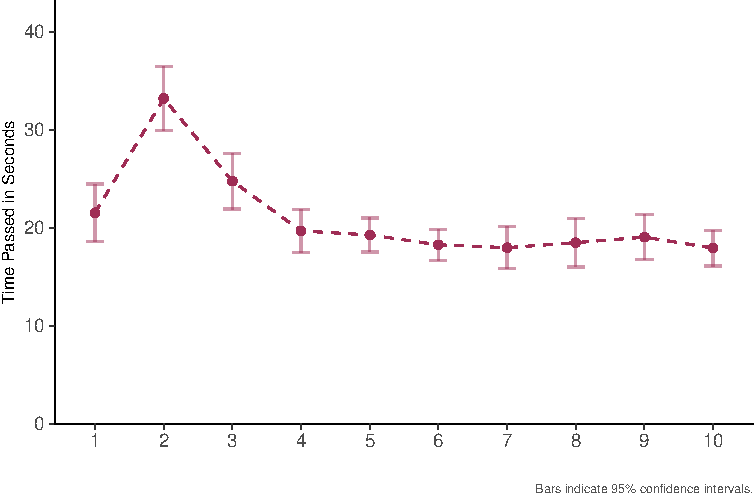
\includegraphics{paper_files/figure-pdf/plotTime-1.pdf}

}

\caption{Average Time Spent for each Contribution per Period}

\end{figure}

\hypertarget{pre-registered-gmtv-replication}{%
\subsection{Pre-registered GMTV
Replication}\label{pre-registered-gmtv-replication}}

\textbf{Result 1.} \emph{The \texttt{NOPUNISH\ 10} treatment of
\citet{GMTV2017} can be replicated because the replication data resemble
the original data with respect to initial and final contributions,
wealth and growth as well as inequality between and within groups.}

This is remarkable given the different sample and language, the
different software and user interface as well as the online setting
during the COVID19 pandemic.

\hypertarget{contributions}{%
\subsubsection{Contributions}\label{contributions}}

First, I ask whether the samples differ with respect to their initial
contributions to the public good. Is our replication sample more
pro-social than the original sample? Figure 1 reveals that it is not.
The distributions of both samples look fairly similar. Both samples
contributed 10 tokens, that is, 50\% of their endowments on average
(median and mean).\footnote{The two-sided rank sum test (comparing
  differences between samples) yields a p-Value of 0.3926 for the mean
  contribution in first round of the game.} Moreover, both samples'
initial contributions resemble initial contributions participants
usually make in the standard game with partner matching.\footnote{See
  Figure 3B in \citet{fehrgaechter2000} (p.989), for instance.} However,
in the dynamic game presented here, we are particularly interested in
the subsequent periods because differences add up exponentially. Do the
two groups remain similar over the course of time?

\begin{figure}

{\centering 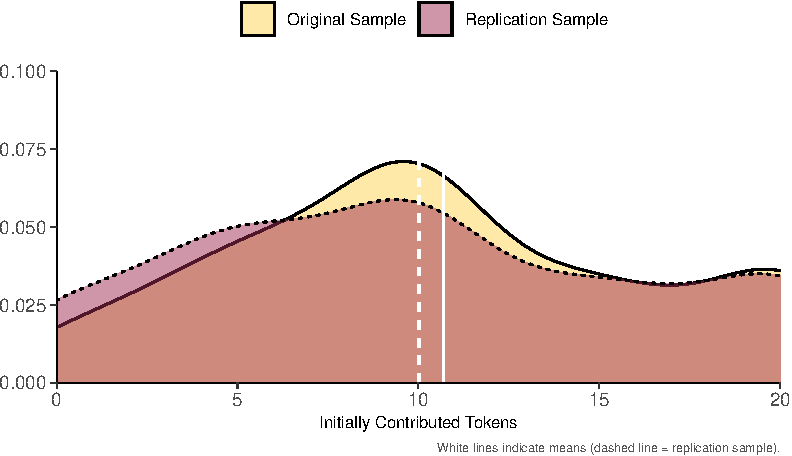
\includegraphics{paper_files/figure-pdf/firstRoundViz-1.pdf}

}

\caption{Individual contributions to the dynamic public good in the
first period}

\end{figure}

In particular, do the two samples' contributions follow the same path
over the 10 periods they played? The answer is \emph{no}. Figure 2
illustrates that the samples make similar contributions at the beginning
and the end of the game but behave differently in between. More
precisely, the left panel--depicting the average contributions in
absolute terms--shows that the original sample contributed substantially
more than the replication sample \emph{in all but the first and last
periods}. For this reason, the original sample's behavior differs from
the replication sample's behavior in two aspects: it contributes more
and exhibits a considerable drop in the last period (whereas the
replication sample's contributions flatten).

Note that increasing contributions over time imply increasing endowments
over time. Hence, absolute contributions do not us much about the
willingness to cooperate. For this reason, the right panel in Figure 2
shows the average \emph{share of endowments contributed} over time. Both
samples exhibit a similar pattern: they decline and do not stabilize.
However, both samples also differ with respect to one aspect: the
replication sample's share of contributions declines faster.

\begin{figure}

{\centering 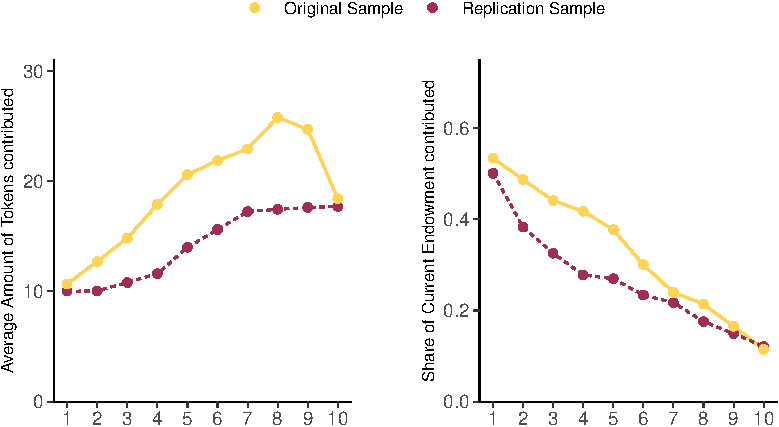
\includegraphics{paper_files/figure-pdf/plotShareOfContributions-1.pdf}

}

\caption{The average amount of tokens contributed over time in
treatments.}

\end{figure}

Again, both samples' behavior resembles the contributions participants
usually make in the standard game with partner matching: contributions
equal approximately half of endowments in the very first period and
decrease to around 10\% of endowments by the last period.\footnote{The
  right panel is thus, comparable to the visualizations \emph{and
  results} in the standard game. See, for instance, Figure 1B in
  \citet{fehrgaechter2000} (p.986).} In the dynamic game presented here,
however, different paths lead to different levels of wealth -- even if
they share the same start- and end-points. I am thus, more interested in
the contributions' implications for wealth generation and growth.

\hypertarget{wealth-creation}{%
\subsubsection{Wealth Creation}\label{wealth-creation}}

How do the different contribution-paths translate into
wealth?\footnote{To measure wealth and growth, I define a variable
  called \emph{stock} which sums the endowments of all participants in a
  given group at the end of the round (that is, after the contributions
  have been made, multiplied and redistributed).} Given that the
original sample contributed more in most of the periods, one would
expect the respective groups to be considerably more wealthy. Figure 3
indicates just that. The grey lines show that an average group in the
original sample accumulated about 478 tokens. In contrast, an average
group in the replication sample accumulated about 380 tokens. This
difference is insignificant at conventional levels\footnote{The
  two-sided rank sum test (comparing differences between samples) yields
  a p-Value of 0.1356 for the mean stock in last round of the game.}
though.

\begin{figure}

{\centering 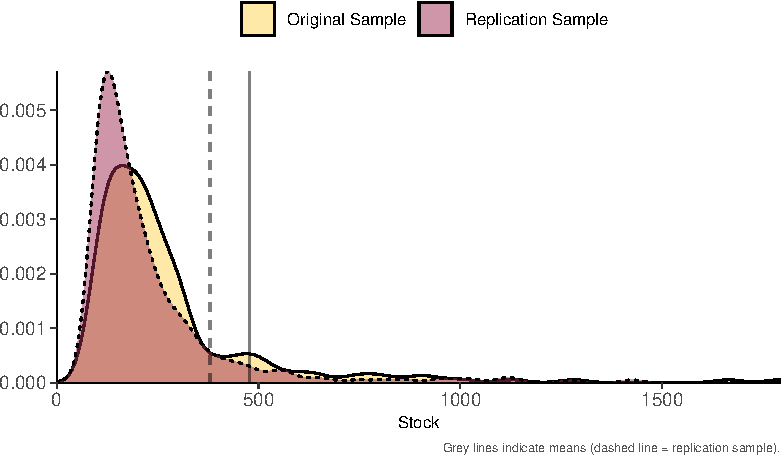
\includegraphics{paper_files/figure-pdf/stockDistributionViz-1.pdf}

}

\caption{Groups' income at the end of the game}

\end{figure}

Although there clearly is growth, groups do not realize the maximal
potential efficiency: under full cooperation, a group can accumulate at
least 4613 tokens or EUR 230. This is depicted in the left panel of
Figure 4, where one can see the average wealth over time by sample. The
panel illustrates for both samples that growth was continuous and
surprisingly linear, given the exponential character of the game's
design. To sum up, the contribution behavior differed between samples.
In contrast, neither the eventual wealth nor the corresponding growth
paths differed. Differences in contribution behavior did, thus, not
translate in significantly different wealth outcomes.

Why? Perhaps because the heterogeneity within samples and across groups
has been too large to \emph{detect} a significant difference. The right
panel of Figure 4 depicts heterogeneity: In the replication sample, the
richest group earned 1425 tokens (which is about 1781\% of the initial
endowment) whereas the poorest group ends up with 92 tokens (115\%).
More broadly, the replication sample is characterized by inequality
between groups (\(SD_{Replication} =\) 336.06). The same holds true for
the original sample (\(SD_{Original} =\) 393.58). Hence, the
heterogeneity across groups does not differ between samples, which is
remarkable because the replication sample was drawn from a more
heterogeneous (non-convenience sample). Does it differ within groups?

\begin{figure}

{\centering 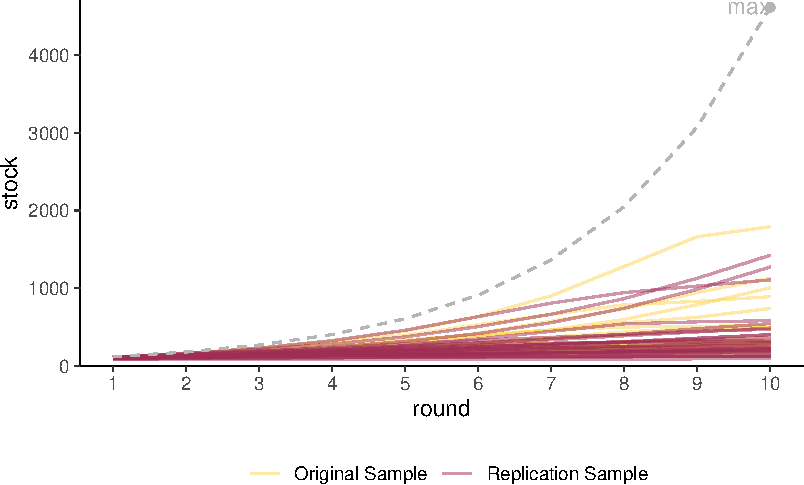
\includegraphics{paper_files/figure-pdf/growthHeterogeneityViz-1.pdf}

}

\caption{Average wealth over time across samples.}

\end{figure}

\hypertarget{inequality}{%
\subsubsection{Inequality}\label{inequality}}

Given the different samples and the possibility of endogenous
growth--which essentially is the main feature of the game--I ask whether
and how the inequality grows \emph{within} groups. Figure 5 illustrates
that inequality did grow: at the end of the game, the original and the
replication groups exhibit an average Gini coefficient of 0.23 and 0.22,
respectively.\footnote{The two-sided rank sum test (comparing
  differences between samples) yields a p-Value of 0.6059 for the mean
  Gini coefficient in last round of the game.} Because every participant
started with the same initial endowment (in \emph{Period 0}, so to
speak), every group started equally--with a Gini coefficient equaling
zero.

Figure 6 shows that this initial state of equality ended with the first
period already: both samples exhibit a stark incline in inequality
before the second period started. From then on, the respective Gini
coefficients grew slowly but continuously -- for both samples.

\begin{figure}

{\centering 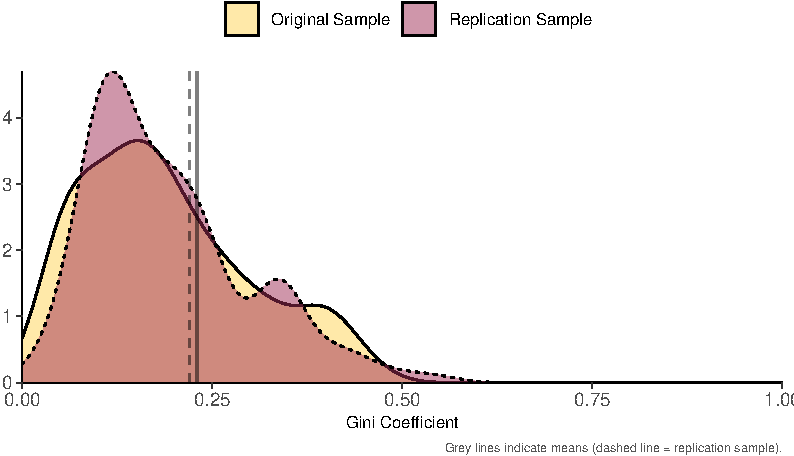
\includegraphics{paper_files/figure-pdf/giniDistributionViz-1.pdf}

}

\caption{Groups' Gini coefficients (within groups) at the end of the
game}

\end{figure}

\begin{figure}

{\centering 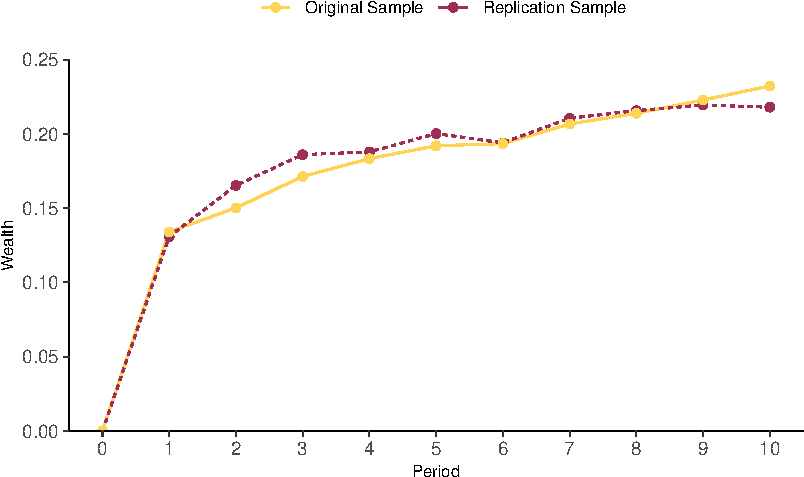
\includegraphics{paper_files/figure-pdf/unnamed-chunk-1-1.pdf}

}

\caption{Average Gini coefficient (within groups) over time across
samples}

\end{figure}

\hypertarget{generalizability}{%
\subsection{Generalizability}\label{generalizability}}

\hypertarget{conclusion}{%
\section{Conclusion}\label{conclusion}}

\hypertarget{appendix}{%
\section{Appendix}\label{appendix}}

\hypertarget{a-pure-replication}{%
\subsection{A: Pure Replication}\label{a-pure-replication}}

\hypertarget{b-growth-and-inequality-exploratory}{%
\subsection{\texorpdfstring{B: Growth \emph{and} Inequality
(exploratory)}{B: Growth and Inequality (exploratory)}}\label{b-growth-and-inequality-exploratory}}

In contrast to \citet{GMTV2017}, I did not ask how rich and poor groups
differ. Instead, I was wondering, whether equal groups are wealthier.
More precisely, does the Gini coefficient correlate with growth and
wealth creation? To answer that question, Figure 7 applies a median
split showing equal and unequal groups' wealth over time.

\begin{figure}

{\centering 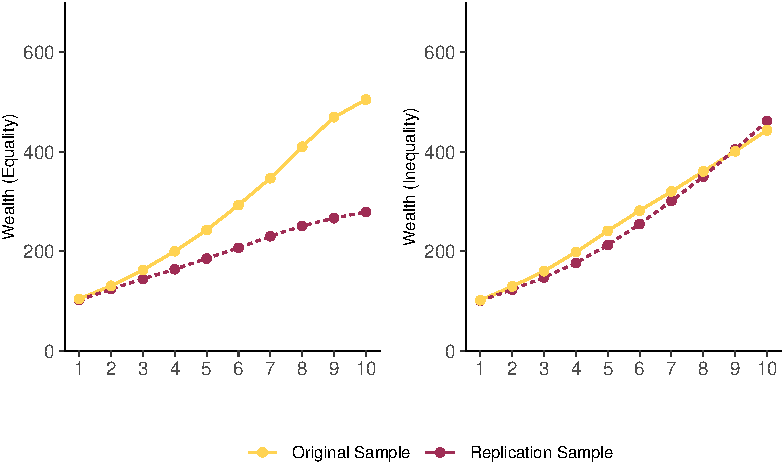
\includegraphics{paper_files/figure-pdf/plotStockByGini-1.pdf}

}

\caption{Average wealth over time across treatments.}

\end{figure}


  \bibliography{../biblio.bib}


\end{document}
